\documentclass{standalone}
\usepackage{pgfplots}
\pgfplotsset{compat=1.8}
\usepackage{mathtools}
\usepackage{tikz}
\begin{document} 

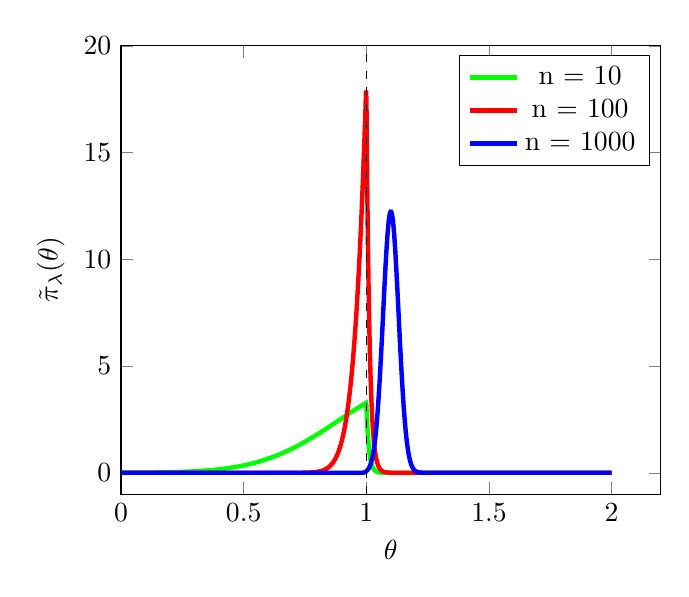
\begin{tikzpicture}
 \begin{axis}[
   scaled ticks=false,
   xmin=0,
   ymin=-1,
   ymax=20,
   xlabel= $\theta$,
   ylabel= $\tilde{\pi}_{\lambda}(\theta)$,
   ]
    \addplot[domain=0:2, green, smooth,ultra thick, samples= 1000] {
     4* exp(-10*(x-1.2)^2/2)  * exp( - 100* (x>1)*(x-1))
    };

  \addplot[domain=0:2, red, smooth,ultra thick, samples= 1000] {
     135* exp(-100*(x-1.2)^2/2) * exp( - 100 * (x>1)*(x-1))
    };

    \addplot[domain=0:2, blue, smooth, ultra thick, samples= 1000] {
     40000000* exp(-1000*(x-1.2)^2/2) * exp( - 100 * (x>1)*(x-1))
    };
  

          \addplot +[mark=none, dashed] coordinates {(1, -1) (1, 20)};
  \addlegendentry{n = 10}
\addlegendentry{n = 100}
\addlegendentry{n = 1000}
\end{axis}
\end{tikzpicture}
\end{document}